\documentclass[a4paper]{article}

\usepackage{inputenc}
\usepackage[british,UKenglish]{babel}
\usepackage{amsmath}
%\usepackage{titlesec}
\usepackage{color}
\usepackage{graphicx}
\usepackage{fancyref}
\usepackage{hyperref}
\usepackage{float}
\usepackage{scrextend}
\usepackage{setspace}
\usepackage{xargs}
\usepackage{multicol}
\usepackage{nameref}

\usepackage{sectsty}
\usepackage{multicol}
\usepackage{multirow}
\usepackage[procnames]{listings}
\usepackage{appendix}

\newcommand\tab[1][1cm]{\hspace*{#1}}
\hypersetup{colorlinks=true, linkcolor=black}
\interfootnotelinepenalty=10000

\newcommand{\cleancode}[1]{\begin{addmargin}[3em]{3em}\texttt{\textcolor{cleanOrange}{#1}}\end{addmargin}}
\newcommand{\cleanstyle}[1]{\text{\textcolor{cleanOrange}{\texttt{#1}}}}


\usepackage[colorinlistoftodos,prependcaption,textsize=footnotesize]{todonotes}
\newcommandx{\commred}[2][1=]{\textcolor{Red}
{\todo[linecolor=red,backgroundcolor=red!25,bordercolor=red,#1]{#2}}}
\newcommandx{\commblue}[2][1=]{\textcolor{Blue}
{\todo[linecolor=blue,backgroundcolor=blue!25,bordercolor=blue,#1]{#2}}}
\newcommandx{\commgreen}[2][1=]{\textcolor{OliveGreen}{\todo[linecolor=OliveGreen,backgroundcolor=OliveGreen!25,bordercolor=OliveGreen,#1]{#2}}}
\newcommandx{\commpurp}[2][1=]{\textcolor{Plum}{\todo[linecolor=Plum,backgroundcolor=Plum!25,bordercolor=Plum,#1]{#2}}}

\def\code#1{{\tt #1}}

\def\note#1{\noindent{\bf [Note: #1]}}

\makeatletter
%% The "\@seccntformat" command is an auxiliary command
%% (see pp. 26f. of 'The LaTeX Companion,' 2nd. ed.)
\def\@seccntformat#1{\@ifundefined{#1@cntformat}%
   {\csname the#1\endcsname\quad}  % default
   {\csname #1@cntformat\endcsname}% enable individual control
}
\let\oldappendix\appendix %% save current definition of \appendix
\renewcommand\appendix{%
    \oldappendix
    \newcommand{\section@cntformat}{\appendixname~\thesection\quad}
}
\makeatother


% "define" Scala
\usepackage[T1]{fontenc}  
\usepackage[scaled=0.82]{beramono}  
\usepackage{microtype} 

\sbox0{\small\ttfamily A}
\edef\mybasewidth{\the\wd0 }

\lstdefinelanguage{scala}{
  morekeywords={abstract,case,catch,class,def,%
    do,else,extends,false,final,finally,%
    for,if,implicit,import,match,mixin,%
    new,null,object,override,package,%
    private,protected,requires,return,sealed,%
    super,this,throw,trait,true,try,%
    type,val,var,while,with,yield},
  sensitive=true,
  morecomment=[l]{//},
  morecomment=[n]{/*}{*/},
  morestring=[b]",
  morestring=[b]',
  morestring=[b]"""
}

\usepackage{color}
\definecolor{dkgreen}{rgb}{0,0.6,0}
\definecolor{gray}{rgb}{0.5,0.5,0.5}
\definecolor{mauve}{rgb}{0.58,0,0.82}

% Default settings for code listings
\lstset{frame=tb,
  language=scala,
  aboveskip=3mm,
  belowskip=3mm,
  showstringspaces=false,
  columns=fixed, % basewidth=\mybasewidth,
  basicstyle={\small\ttfamily},
  numbers=none,
  numberstyle=\footnotesize\color{gray},
  % identifierstyle=\color{red},
  keywordstyle=\color{blue},
  commentstyle=\color{dkgreen},
  stringstyle=\color{mauve},
  frame=single,
  breaklines=true,
  breakatwhitespace=true,
  procnamekeys={def, val, var, class, trait, object, extends},
  procnamestyle=\ttfamily\color{red},
  tabsize=2
}

\lstnewenvironment{scala}[1][]
{\lstset{language=scala,#1}}
{}
\lstnewenvironment{cpp}[1][]
{\lstset{language=C++,#1}}
{}
\lstnewenvironment{bash}[1][]
{\lstset{language=bash,#1}}
{}
\lstnewenvironment{verilog}[1][]
{\lstset{language=verilog,#1}}
{}



%代码段设置
\lstset{numbers=left,
basicstyle=\tiny,
numberstyle=\tiny,
keywordstyle=\color{blue!70},
commentstyle=\color{red!50!green!50!blue!50},
frame=single, rulesepcolor=\color{red!20!green!20!blue!20},
escapeinside=``
}

\graphicspath{ {images/} }
\usepackage{ctex}
\usepackage{graphicx}
\usepackage{color,framed}%文本框
\usepackage{listings}
\usepackage{caption}
\usepackage{amssymb}
\usepackage{enumerate}
\usepackage{xcolor}
\usepackage{bm} 
\usepackage{lastpage}%获得总页数
\usepackage{fancyhdr}
\usepackage{tabularx}  
\usepackage{geometry}
\usepackage{minted}
\usepackage{graphics}
\usepackage{subfigure}
\usepackage{float}
\usepackage{pdfpages}
\usepackage{pgfplots}
\pgfplotsset{width=10cm,compat=1.9}
\usepackage{multirow}
\usepackage{footnote}
\usepackage{booktabs}

%-----------------------伪代码------------------
\usepackage{algorithm}  
\usepackage{algorithmicx}  
\usepackage{algpseudocode}  
\floatname{algorithm}{Algorithm}  
\renewcommand{\algorithmicrequire}{\textbf{Input:}}  
\renewcommand{\algorithmicensure}{\textbf{Output:}} 
\usepackage{lipsum}  
\makeatletter
\newenvironment{breakablealgorithm}
  {% \begin{breakablealgorithm}
  \begin{center}
     \refstepcounter{algorithm}% New algorithm
     \hrule height.8pt depth0pt \kern2pt% \@fs@pre for \@fs@ruled
     \renewcommand{\caption}[2][\relax]{% Make a new \caption
      {\raggedright\textbf{\ALG@name~\thealgorithm} ##2\par}%
      \ifx\relax##1\relax % #1 is \relax
         \addcontentsline{loa}{algorithm}{\protect\numberline{\thealgorithm}##2}%
      \else % #1 is not \relax
         \addcontentsline{loa}{algorithm}{\protect\numberline{\thealgorithm}##1}%
      \fi
      \kern2pt\hrule\kern2pt
     }
  }{% \end{breakablealgorithm}
     \kern2pt\hrule\relax% \@fs@post for \@fs@ruled
  \end{center}
  }
\makeatother
%------------------------代码-------------------
\usepackage{xcolor} 
\usepackage{listings} 
\lstset{ 
breaklines,%自动换行
basicstyle=\small,
escapeinside=``,
keywordstyle=\color{ blue!70} \bfseries,
commentstyle=\color{red!50!green!50!blue!50},% 
stringstyle=\ttfamily,% 
extendedchars=false,% 
linewidth=\textwidth,% 
numbers=left,% 
numberstyle=\tiny \color{blue!50},% 
frame=trbl% 
rulesepcolor= \color{ red!20!green!20!blue!20} 
}

%-------------------------页面边距--------------
\geometry{a4paper,left=2.3cm,right=2.3cm,top=2.7cm,bottom=2.7cm}
%-------------------------页眉页脚--------------
\usepackage{fancyhdr}
\pagestyle{fancy}
\lhead{\kaishu \leftmark}
% \chead{}
\rhead{\kaishu 并行程序设计实验报告}%加粗\bfseries 
\lfoot{}
\cfoot{\thepage}
\rfoot{}
\renewcommand{\headrulewidth}{0.1pt}  
\renewcommand{\footrulewidth}{0pt}%去掉横线
\newcommand{\HRule}{\rule{\linewidth}{0.5mm}}%标题横线
\newcommand{\HRulegrossa}{\rule{\linewidth}{1.2mm}}
\setlength{\textfloatsep}{10mm}%设置图片的前后间距
%--------------------文档内容--------------------

\begin{document}
\renewcommand{\contentsname}{目\ 录}
\renewcommand{\appendixname}{附录}
\renewcommand{\appendixpagename}{附录}
\renewcommand{\refname}{参考文献} 
\renewcommand{\figurename}{图}
\renewcommand{\tablename}{表}
\renewcommand{\today}{\number\year 年 \number\month 月 \number\day 日}

%-------------------------封面----------------
\begin{titlepage}
    \begin{center}
    
\includegraphics[width=0.8\textwidth]{NKU.png}\\[1cm]
    \vspace{20mm}
		\textbf{\huge\textbf{\kaishu{计算机学院}}}\\[0.5cm]
		\textbf{\huge{\kaishu{并行程序设计实验报告}}}\\[2.3cm]
		\textbf{\Huge\textbf{\kaishu{作业二:体系结构及性能相关测试}}}

		\vspace{\fill}
    
    % \textbf{\Large \textbf{并行程序设计期末实验报告}}\\[0.8cm]
    % \HRule \\[0.9cm]
    % \HRule \\[2.0cm]
    \centering
    \textsc{\LARGE \kaishu{姓名\ :\ 熊宇轩}}\\[0.5cm]
    \textsc{\LARGE \kaishu{学号\ :\ 2010056}}\\[0.5cm]
    \textsc{\LARGE \kaishu{专业\ :\ 计算机科学与技术}}\\[0.5cm]
    
    \vfill
    {\Large 2022年3月13日}
    \end{center}
\end{titlepage}

\renewcommand {\thefigure}{\thesection{}.\arabic{figure}}%图片按章标号
\renewcommand{\figurename}{图}
\renewcommand{\contentsname}{目录}  
\cfoot{\thepage\ of \pageref{LastPage}}%当前页 of 总页数


% 生成目录
\clearpage
\tableofcontents
\newpage

%--------------------------Title--------------------------------
\section{实验目标}
   \begin{enumerate}
   \item 以矩阵每一列与向量的内积为例,通过编写代码实践cache优化算法。
   \item 以求数组累加和为例,通过编写代码实践两路链式相加、循环展开和递归相加等超标量优化算法。
   \item 利用prof和uprof等工具,通过运行计时和事件计数的方法,量化分析普通算法和优化算法之间的性能差异。
   \end{enumerate}
\section{实验环境}
   \subsection{X86平台}
      X86平台使用的是一台笔记本电脑,具体参数如下:
      \begin{minted}[mathescape,
                     linenos,
                     numbersep=5pt,
                     gobble=2,
                     frame=lines,
                     framesep=2mm,
                     highlightcolor=green!40]{bash}
         suhipek@suhipek-BOHK-WAX9X:~$ lscpu
         Architecture:                    x86_64
         CPU(s):                          8
         L1d cache:                       128 KiB
         L1i cache:                       256 KiB
         L2 cache:                        2 MiB
         L3 cache:                        4 MiB
      \end{minted}
      其中显示的L1数据和指令缓存为四个CPU核心缓存数量的总和,每个CPU核心实际的数据缓存大小为32KB。
      \subsection{ARM平台}
      ARM平台使用课程提供的服务器,具体参数如下:
      \begin{minted}[mathescape,
                     linenos,
                     numbersep=5pt,
                     gobble=2,
                     frame=lines,
                     framesep=2mm,
                     highlightcolor=green!40]{bash}
         [s2010056@master screenFetch]$ lscpu
         Architecture:          aarch64
         CPU(s):                96
         L1d 缓存:          64K
         L1i 缓存:          64K
         L2 缓存:           512K
         L3 缓存:           49152K
      \end{minted}
\newpage
\section{实验设计及分析}
   \subsection{cache优化}
      \subsubsection{实验设计}

      \subsubsection{实验分析}
      矩阵列向量点积实验运行计时的结果如下图所示,其中,矩阵行列数在实验中以16为步进。
      \begin{figure}[!htbp]
         \centering
         \subfigure[ARM平台]{
         \begin{minipage}[t]{0.5\linewidth}
         \centering
         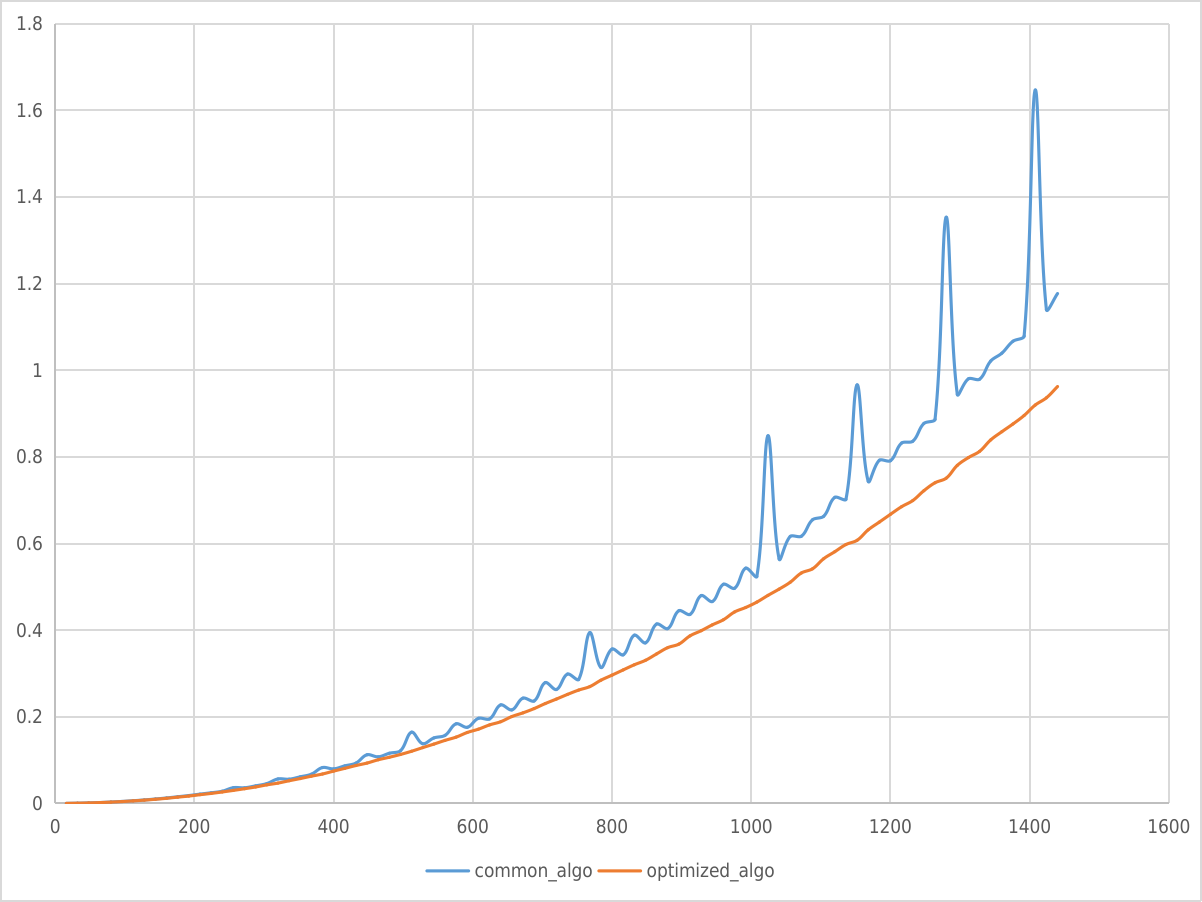
\includegraphics[width=3.2in]{fig/ARM_mat_timing.png}
         \label{fig:diff1}
         \end{minipage}%
         }%
         \subfigure[X86平台]{
         \begin{minipage}[t]{0.5\linewidth}
         \centering
         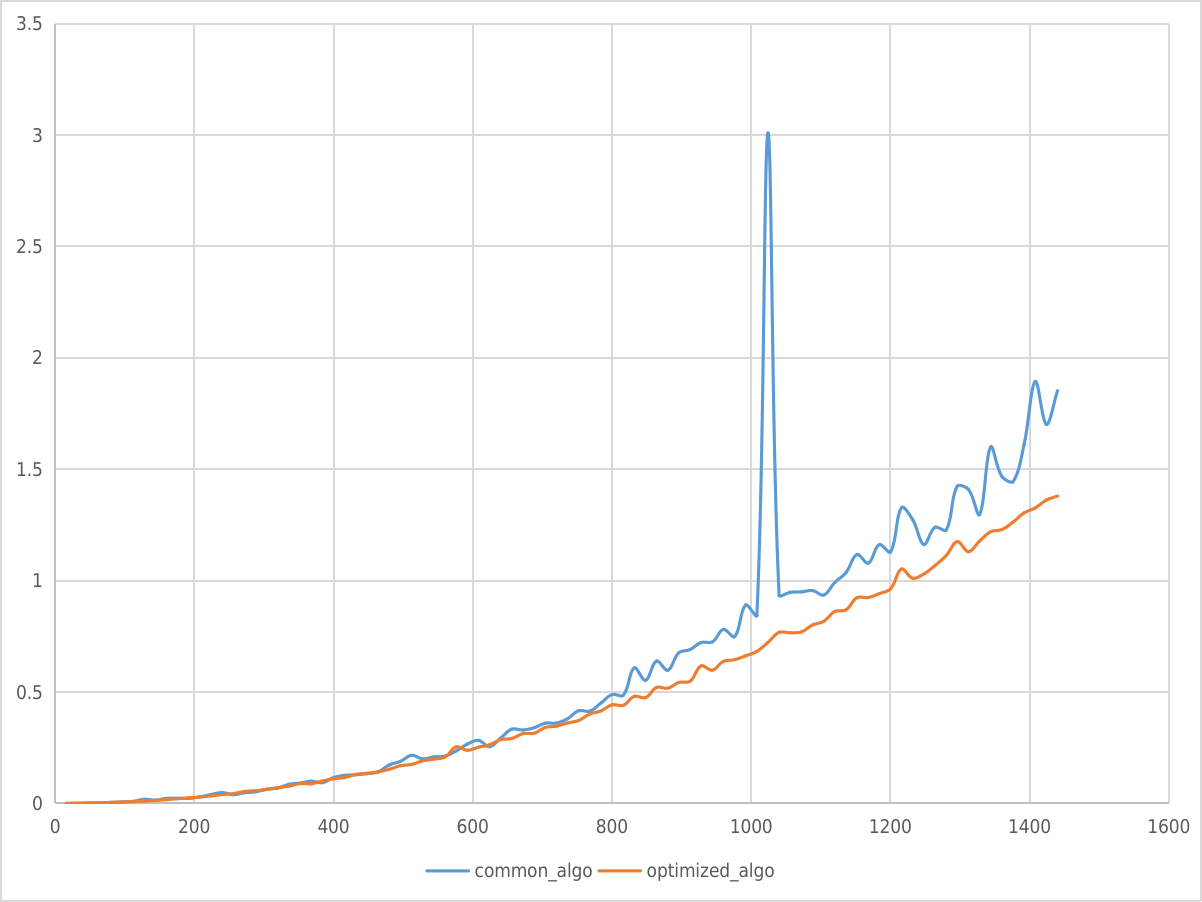
\includegraphics[width=3.2in]{fig/X86_mat_timing.png}
         \end{minipage}%
         }
         \centering
         \caption{矩阵列向量点积(矩阵行/列数-运行时间)(单位/秒)}
         \label{fig:mat_timing}
      \end{figure}
      \begin{table}[!htbp]
         \centering
         \begin{tabular}{@{}lllll@{}}
         \toprule
         函数              & \begin{tabular}[c]{@{}l@{}}L1-dcache-\\ load-misses\end{tabular} & L1-dcache-loads & \begin{tabular}[c]{@{}l@{}}L1-dcache-\\ store-misses\end{tabular} & L1-dcache-stores \\ \midrule
         common\_algo    & 86.84\%               & 50.00\%         & 86.83\%                & 50.00\%          \\
         optimized\_algo & 13.13\%               & 49.99\%         & 13.12\%                & 49.99\%          \\
         事件总数            & 30070924              & 3570518704      & 30070932               & 3570537681       \\ \bottomrule
         \end{tabular}
         \caption{ARM平台下矩阵列向量与向量点积的perf事件计数结果}
         \label{table:t_ARM_cache}
         \end{table}
         
         \begin{table}[!htbp]
         \centering
         \begin{tabular}{@{}llll@{}}
         \toprule
         函数              & L1-dcache-load-misses & L1-dcache-loads & L1-dcache-prefetches \\ \midrule
         common\_algo    & 93.55\%               & 50.61\%         & 92.10\%              \\
         optimized\_algo & 6.33\%                & 49.23\%         & 7.67\%               \\
         事件总数            & 105630435             & 3161589638      & 80585651             \\ \bottomrule
         \end{tabular}
         \caption{X86平台下矩阵列向量与向量点积的perf事件计数结果}
         \label{table:t_x86_cache}
         \end{table}
   \subsection{}
      \subsubsection{实验设计}

      \subsubsection{实验分析}
      累加实验运行计时的结果如下图所示
      \begin{figure}[!htbp]
      \centering
      \subfigure[ARM平台]{
      \begin{minipage}[t]{0.5\linewidth}
      \centering
      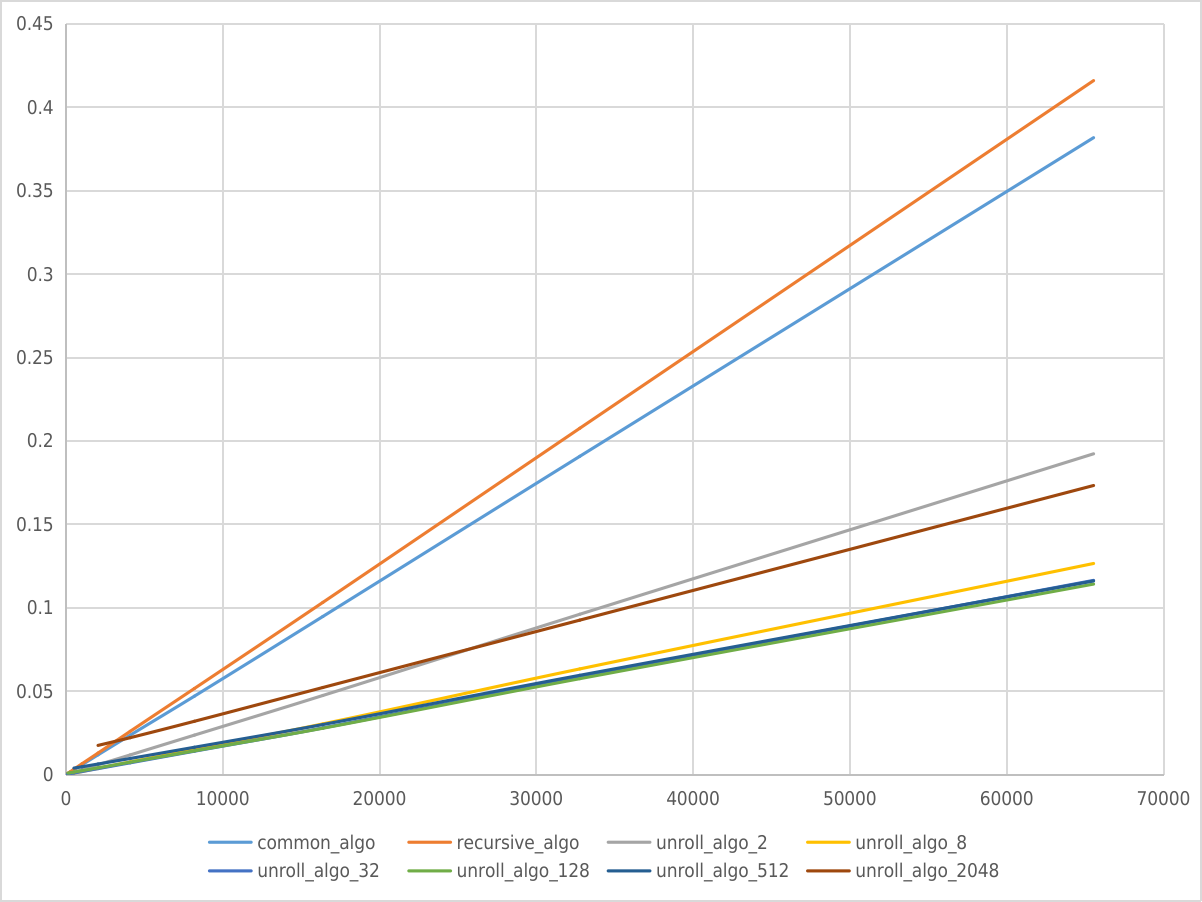
\includegraphics[width=3.2in]{fig/ARM_sum_timing.png}
      \label{fig:diff1}
      \end{minipage}%
      }%
      \subfigure[X86平台]{
      \begin{minipage}[t]{0.5\linewidth}
      \centering
      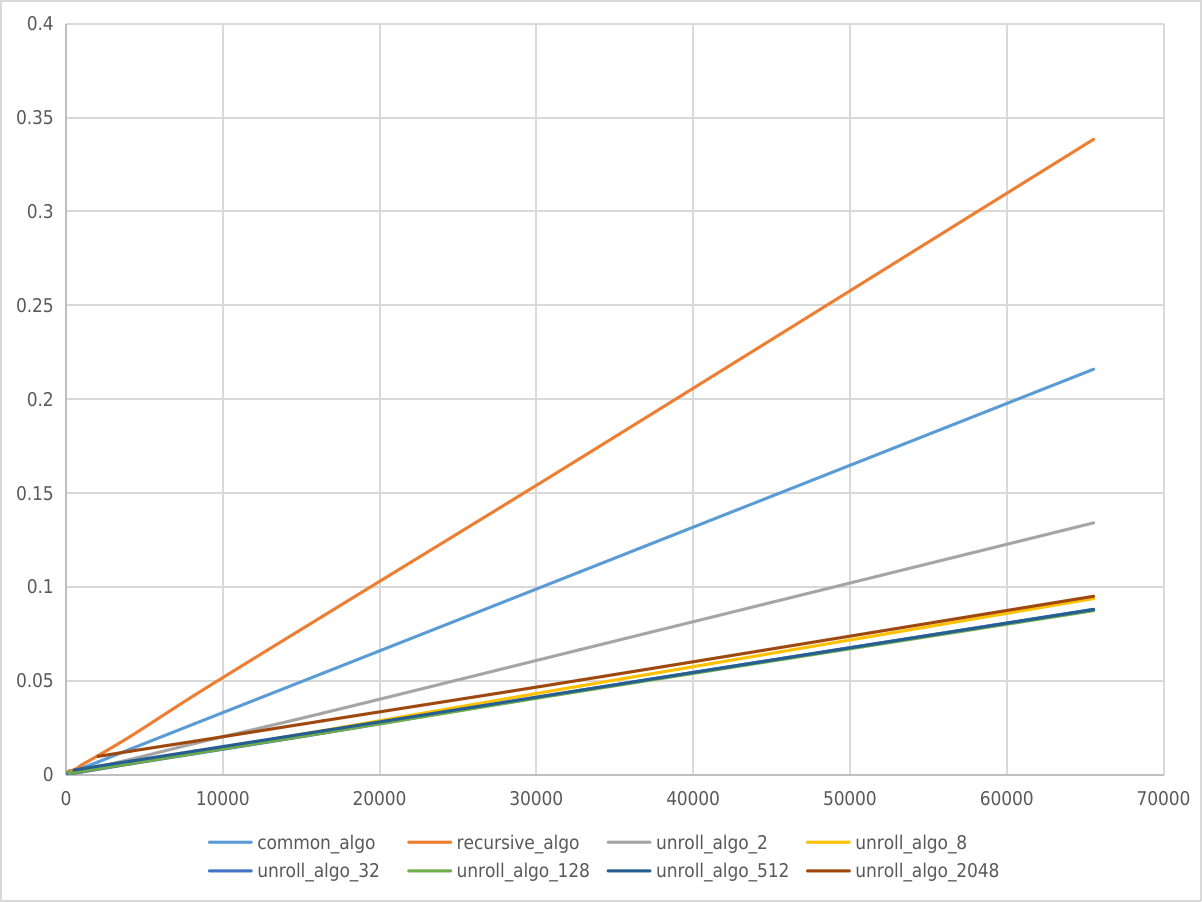
\includegraphics[width=3.2in]{fig/X86_sum_timing.png}
      \end{minipage}%
      }
      \centering
      \caption{累加(输入数组长度-运行时间)(单位/秒)}
      \label{fig:sum_timing}
      \end{figure}
      \begin{table}[!htbp]
         \centering
         \begin{tabular}{@{}llllll@{}}
         \toprule
         \begin{tabular}[c]{@{}l@{}}优化方法或\\ 循环展开的层数\end{tabular} & cycles       & instructions & CPI    & \begin{tabular}[c]{@{}l@{}}L1-dcache-\\ load-misses\end{tabular} & \begin{tabular}[c]{@{}l@{}}L1-icache-\\ load-misses\end{tabular} \\ \midrule
         不优化                                                     & 13.41\%      & 9.19\%       & 0.6296 & 8.24\%                                                           & 0.00\%                                                           \\
         递归                                                      & 15.55\%      & 18.67\%      & 0.3594 & 15.01\%                                                          & 0.00\%                                                           \\
         2                                                       & 6.73\%       & 7.07\%       & 0.4107 & 6.50\%                                                           & 0.00\%                                                           \\ 
         32                                                      & 4.14\%       & 5.21\%       & 0.3429 & 5.06\%                                                           & 0.00\%                                                           \\
         512                                                     & 4.15\%       & 5.10\%       & 0.3511 & 6.01\%                                                           & 0.00\%                                                           \\
         8192                                                    & 9.89\%       & 6.51\%       & 0.6555 & 8.04\%                                                           & 45.59\%                                                          \\
         事件总数                                                    & 122855688833 & 284706374706 & 0.4315 & 633713953                                                        & 2540277364                                                       \\ \bottomrule
         \end{tabular}
         \caption{ARM平台下累加优化算法的perf事件计数结果}
         \label{table:perf_arm_sum}
         \end{table}
         
         \begin{table}[!htbp]
         \centering
         \begin{tabular}{@{}llllll@{}}
         \toprule
         \begin{tabular}[c]{@{}l@{}}优化方法或\\ 循环展开的层数\end{tabular} & cycles      & instructions & CPI    & \begin{tabular}[c]{@{}l@{}}L1-dcache-\\ load-misses\end{tabular} & \begin{tabular}[c]{@{}l@{}}L1-icache-\\ load-misses\end{tabular} \\ \midrule
         不优化                           & 11.81\%     & 6.92\%       & 0.6762 & 5.70\%                                                           & 2.10\%                                                           \\
         递归                            & 22.60\%     & 17.53\%      & 0.5108 & 16.13\%                                                          & 4.13\%                                                           \\
         2                             & 7.24\%      & 6.70\%       & 0.4281 & 5.51\%                                                           & 1.46\%                                                           \\
         32                            & 4.84\%      & 5.76\%       & 0.3329 & 5.36\%                                                           & 1.30\%                                                           \\
         512                           & 4.64\%      & 5.59\%       & 0.3288 & 5.38\%                                                           & 2.10\%                                                           \\
         8192                          & 5.05\%      & 5.69\%       & 0.3516 & 10.48\%                                                          & 61.37\%                                                          \\
         事件总数                          & 52560137817 & 132651641398 & 0.3962 & 889797839                                                        & 60817536                                                                 \\ \bottomrule
         \end{tabular}
         \caption{X86平台下累加优化算法的perf事件计数结果}
         \label{table:perf_X86_sum}
         \end{table}
\newpage}

\subsection{Cache优化}
从运行计时的结果图\ref{fig:mat_timing}可以看出,当输入数据规模超出某一个值后,优化的行主访问模式相较于列主访问,在运算时间上产生了较大的优势。根据事件计数的结果表\ref{table:t_ARM_cache},ARM平台上,在L1-dcache-loads、L1-dcache-stores事件数量相差无几的前提下,列主访问的平凡算法所产生的L1-dcache-load-misses、L1-dcache-store-misses的事件数量是行主访问的优化算法的6倍以上。这表明了,列主访问不能最大化发挥cache的潜能,这应该也是行主访问在运行计时上优于列主访问的原因。

\subsection{超标量优化}
从运行计时的结果图\ref{fig:sum_timing}可以看出,无论是两路链式,还是循环展开,其运行速度都优于平凡算法,根据表\ref{table:perf_arm_sum}可以看出,平凡算法的CPI为0.6296,两路链式的CPI为0.4107,而32路链式的CPI为0.3429,这表明在一定范围内,通过增加单次循环中所执行的操作数来进行循环展开的优化,是可以充分利用CPU流水线的设计,得到一定的性能收益的

\subsection{其它问题分析}
\subsubsection{列向量点积数据中的尖峰}
不难注意到,在图\ref{fig:mat_timing}中,ARM平台平凡算法的数据有四个明显的尖峰,除了这四个尖峰外,整个曲线表现出有规律的上下波动。经过几次重复实验后,发现曲线上相近的位置上依然存在着尖峰。并且查看尖峰对应的输入矩阵行数,发现它们恰巧对应着1024、1152、1280、1408(delta=128)这四个数值。

在ARM平台上perf事件计数测量时发现,当矩阵行数为1024时,L1-dcache-load-misses的事件数量比矩阵行数为1025时多了60\%。进一步分析汇编代码,发现这些事件基本都集中在提取矩阵mat[j][i]这个操作上。查阅资料后发现,这个问题可能和cache的结构有关,在鲲鹏920处理器上,Cache划分成了128字节的小块,这种小块被称为Cache Line,而同一个Cache Line是不可被同时访问的。由于出现尖峰的曲线对应的是列主访问的算法,行列数为整倍数的矩阵导致每次从Cache中提取元素都需要跨行访问,导致了额外的开销。也有可能由于超标量的特性,可能存在两条指令同时需要修改同一个Cache Line中的内容的情况,这就造成了伪共享(false sharing)现象,从而导致Cache命中率降低。

\begin{figure}[!htbp]
    \centering
    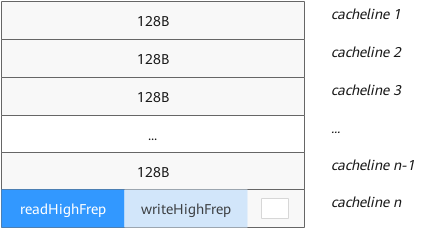
\includegraphics[width=3in]{fig/cache_line.png}
    \caption{Cache的结构 - Cache Line\cite{cacheline}}
    \label{fig:cache_line}
\end{figure}

而在X86平台上,平凡算法的曲线上也存在一个尖峰。perf分析发现,矩阵行数为1024时,branch-misses事件数量比比矩阵行数为1025时多了50\%,而L1-dcache-load-misses的事件数量则是相近的。这可能是由于不同平台的PMU(性能测量单元)或者Cache结构存在着差别,而X86平台上出现尖峰的原因与ARM平台是类似的。也可能是4M的L3 Cache被矩阵占满后,数据存储导致了额外的开销。

其实,在程序性能优化中,Cache Line对齐是非常重要的一环,通过对数据结构的优化,程序可以获得可观的性能提升。

\subsubsection{ARM和X86平台的区别}
不难注意到,在矩阵列向量点积的实验中,ARM平台的总体Cache命中率要比X86平台高很多(99.158\% vs 96.659\%),这可能是由于ARM平台有着更加智能的Cache访问模式,也可能仅仅是因为ARM平台的L1缓存更大(64KB vs 32KB)。此外,不难发现ARM平台的累加的实验的运行时间要比X86平台长得多,这很有可能是因为指令集架构的不同导致的。

\subsubsection{循环展开的层数}
在图\ref{fig:sum_timing}中,可以发现并不是循环展开的路数越多,算法的性能就越好。比如在ARM平台上,2路展开就和8192路展开运行的速度差不多。根据表\ref{table:perf_arm_sum}和表\ref{table:perf_X86_sum}的perf性能分析发现,8192路展开产生了大量的L1-dcache-load-misses和L1-icache-load-misses事件,导致了性能的降低。

导致这现象一方面的原因是,展开循环后的每一行代码依然会产生一定的misses事件,积少成多便降低了Cache命中率。此外,输入数据达到一定规模后,L1 Cache便不再能存下所有的数据了,因此后面的展开会造成大量的性能开销。

这个现象告诉程序设计者们,进行循环展开时的层数也不是越高越好的:展开的层数太高不仅会导致程序体积的变大,还不能给性能带来任何正面的提升。

\subsubsection{递归算法的负优化}
在图\ref{fig:sum_timing}中,显而易见的,递归算法是所有算法中效率最低的一个,这明显是不符合直觉的。分析表\ref{table:perf_arm_sum}和表\ref{table:perf_X86_sum}后发现,递归算法产生了大量的L1-dcache-load-misses事件,这很有可能是因为递归算法需要进行大量不连续内存的访问,跨越Cache Line或者Cache Line伪共享很可能是命中率降低的罪魁祸首。

此外,递归算法的代码本身就比平凡算法和多路链式算法要复杂,多出来的变量也很可能造成了不小的额外开销。

\newpage
\bibliographystyle{plain}
\bibliography{reference.bib} 

\end{document}